\chapter{Methodology}
\label{chap:methodology}

This chapter presents the architectural design, training algorithms, inference optimizations, and system integration strategies developed to achieve passive real-time face anti-spoofing on commodity CPU hardware. Building upon the theoretical formulations in Chapter~\ref{chap:theoretical_background} and the curated person-disjoint datasets in Chapter~\ref{chap:data_processing}, every component from neural layer topology to multi-threaded camera scheduling and WebSocket attendance gating is specified in reproducible detail.

\section{Overall Workflow}
\label{sec:overall_workflow}

Figure~\ref{fig:workflow} depicts the end-to-end engineering workflow, organized into an offline model preparation pipeline (Stage~1) and a unified online runtime serving three operational channels (Stage~2).

\begin{figure}[htbp]
\centering
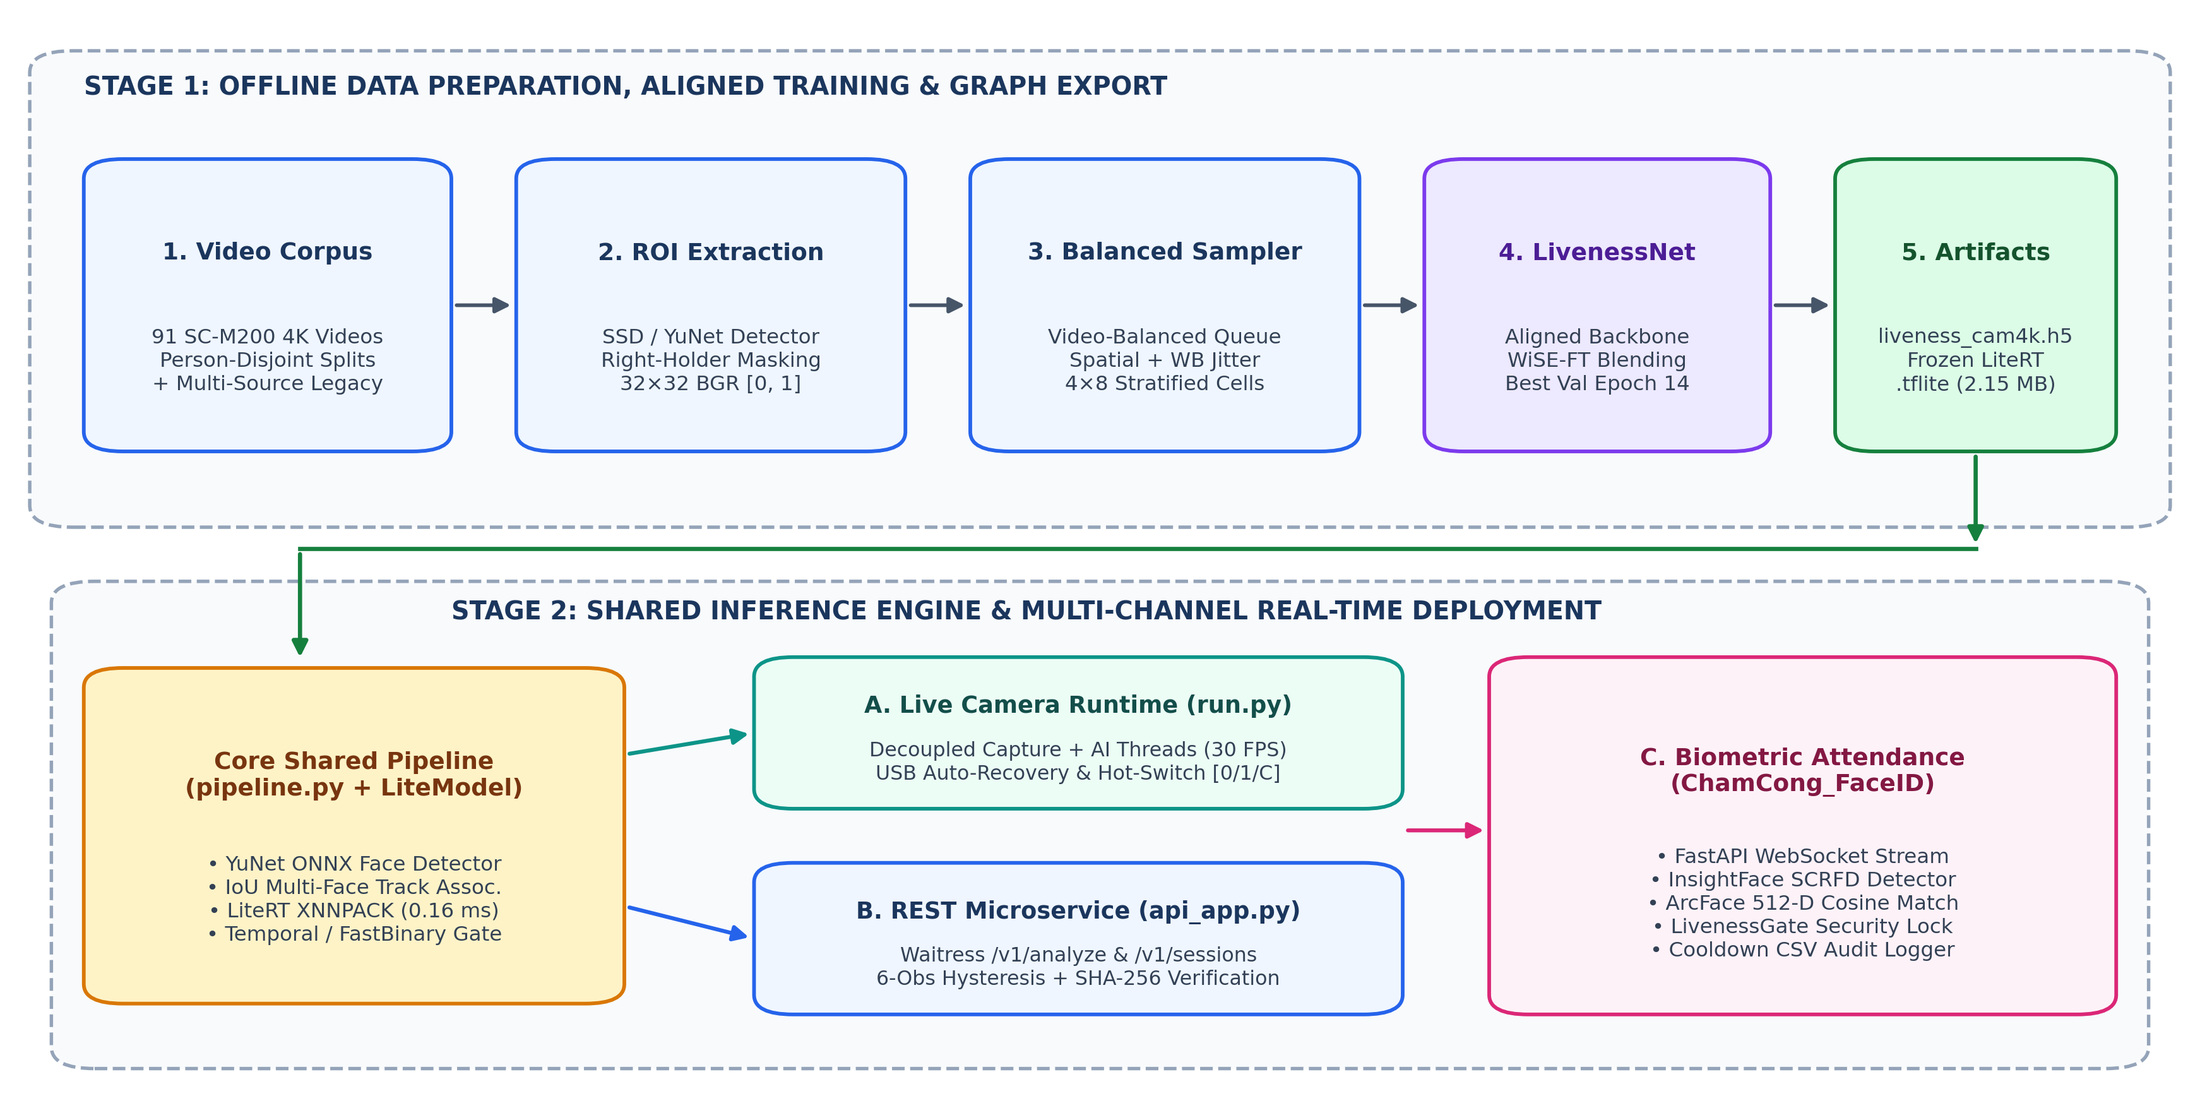
\includegraphics[width=0.98\textwidth]{Images/fig_system_workflow.jpg}
\caption{End-to-end system workflow comprising Stage~1 (offline ROI extraction, balanced training, WiSE-FT head interpolation, and LiteRT export) and Stage~2 (shared CPU inference pipeline powering live camera UI, REST microservice, and biometric attendance verification).}
\label{fig:workflow}
\end{figure}

In \textbf{Stage~1}, person-disjoint raw videos from the SC-M200 \texttt{Cam4K} benchmark and multi-source legacy archives undergo automated ROI localization, presenter-face spatial masking, and six-stage quality filtering to produce normalized $32\times32\times3$ BGR patches. A video-balanced mini-batch generator feeds \texttt{LivenessNet} under geometric and per-channel white-balance jitter. Rather than retraining early spatial filters from scratch on a single sensor, the convolutional feature extractor is anchored to universal multi-source weights while the dense classification head is adapted to the SC-M200 distribution and blended via WiSE-FT~\cite{wortsman2022robust}. The selected Epoch~$14$ checkpoint is serialized both as a standard Keras artifact (\texttt{liveness\_cam4k.h5}) and as a frozen LiteRT flatbuffer (\texttt{liveness\_cam4k.tflite}).

In \textbf{Stage~2}, a single shared inference engine (\texttt{pipeline.py} coupled with \texttt{LiteModel}) executes YuNet ONNX face detection, greedy $\text{IoU}$ multi-face track association, $0.163$~ms XNNPACK CNN scoring, and temporal smoothing. This shared core eliminates training-serving skew across three deployment targets: (A) an interactive $30$~FPS desktop camera monitor (\texttt{run.py}), (B) a stateless/stateful HTTP microservice (\texttt{api\_app.py}), and (C) the \texttt{ChamCong\_FaceID} WebSocket biometric attendance application.

\section{System Design and Architecture}
\label{sec:system_architecture}

\subsection{\texttt{LivenessNet} Convolutional Architecture and Normalization Variants}

To satisfy sub-millisecond CPU latency constraints while preventing subject-identity memorization on $32\times32$ patches, \texttt{LivenessNet} (\texttt{model/livenessnet.py}) adopts a compact VGG-inspired~\cite{simonyan2015very} sequential topology with progressively expanding channel widths ($32 \to 64 \to 128$) and aggressive spatial downsampling ($32 \to 10 \to 5 \to 2$). Figure~\ref{fig:model_architecture} illustrates the block-level tensor flow, and Table~\ref{tab:livenessnet_layers} enumerates every layer, output dimension, and parameter count.

\begin{figure}[htbp]
\centering
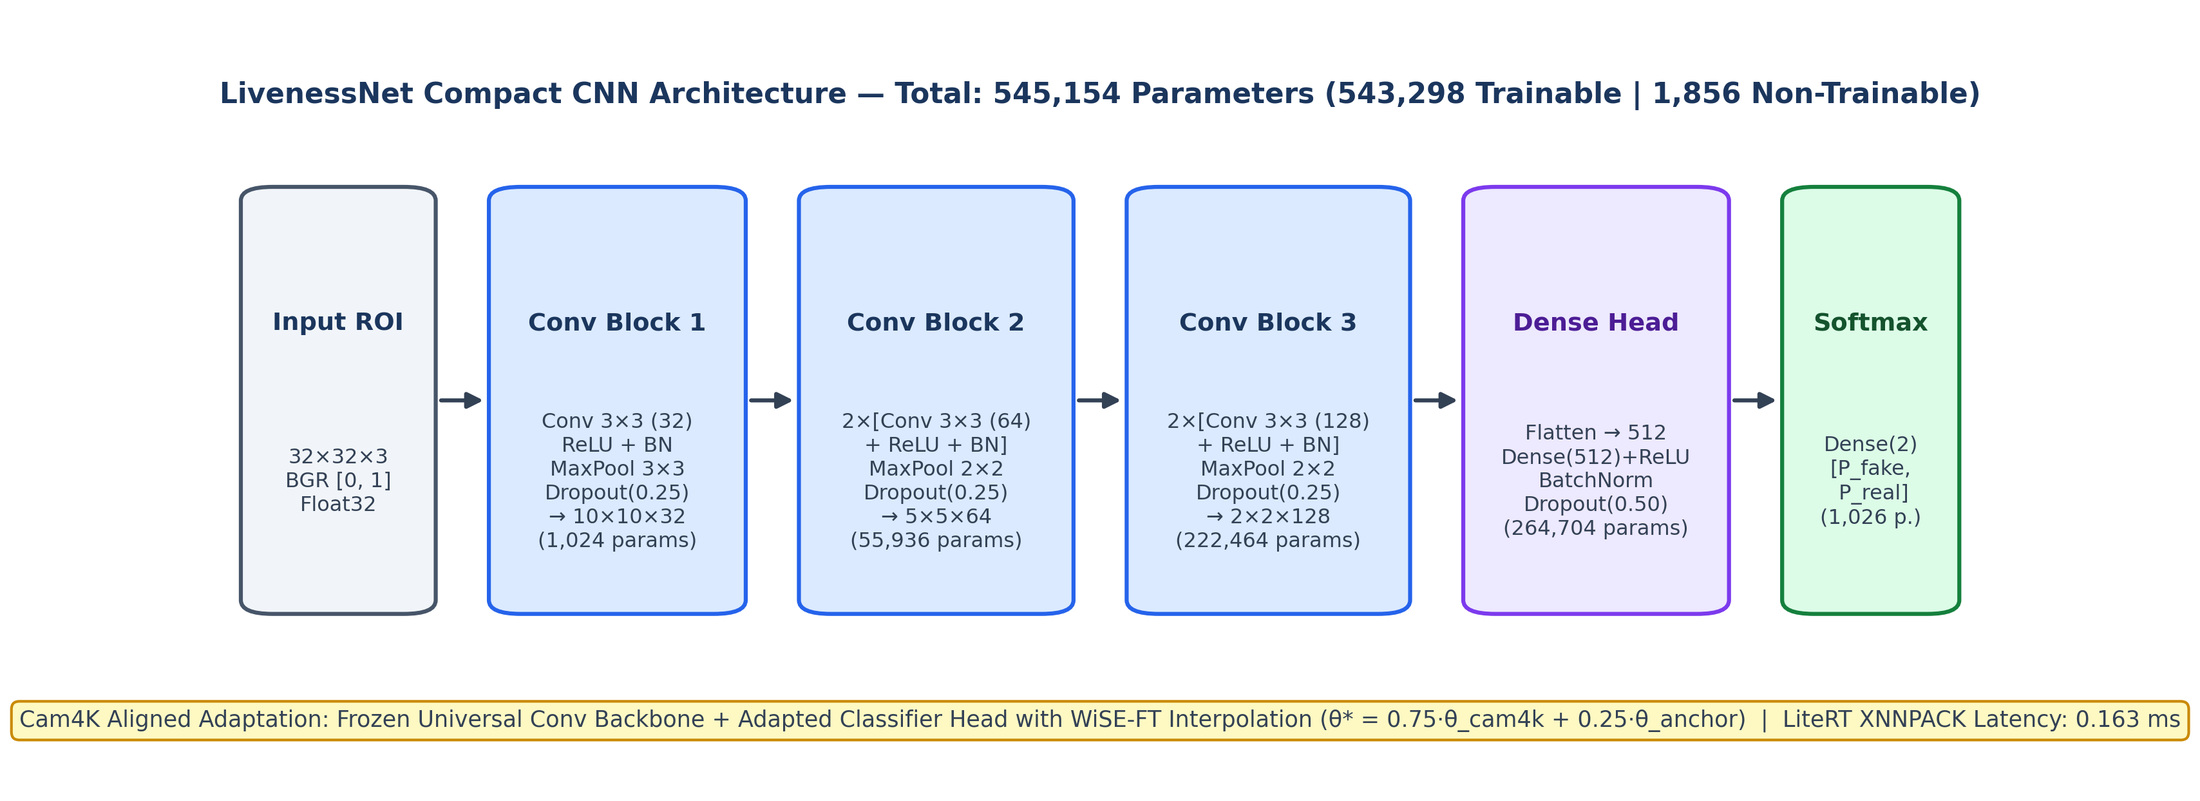
\includegraphics[width=0.98\textwidth]{Images/fig_livenessnet_arch.jpg}
\caption{Block diagram of the $545{,}154$-parameter \texttt{LivenessNet} CNN architecture, highlighting spatial downsampling across three convolutional blocks, the $512$-unit classifier head, and WiSE-FT aligned transfer.}
\label{fig:model_architecture}
\end{figure}

\begin{table}[htbp]
\centering
\caption{Layer-by-layer specification of \texttt{LivenessNet} (input tensor $32 \times 32 \times 3$, channels-last).}
\label{tab:livenessnet_layers}
\small
\begin{tabular}{L{2.3cm}L{3.9cm}L{2.8cm}L{2.3cm}R{2.1cm}}
\toprule
\textbf{Stage} & \textbf{Layer / Operation} & \textbf{Kernel / Config} & \textbf{Output Shape} & \textbf{Parameters} \\
\midrule
Input & Normalized BGR Patch & $\text{float32} \in [0, 1]$ & $32 \times 32 \times 3$ & $0$ \\
\midrule
\multirow{3}{*}{Conv Block 1} & \texttt{Conv2D} + \texttt{ReLU} & $32 \times (3\times3)$, \texttt{same} & $32 \times 32 \times 32$ & $896$ \\
 & \texttt{BatchNormalization} & $\text{axis}=-1$ & $32 \times 32 \times 32$ & $128$ \\
 & \texttt{MaxPooling2D} + \texttt{Dropout} & Pool $3\times3$, $p=0.25$ & $10 \times 10 \times 32$ & $0$ \\
\midrule
\multirow{5}{*}{Conv Block 2} & \texttt{Conv2D} + \texttt{ReLU} & $64 \times (3\times3)$, \texttt{same} & $10 \times 10 \times 64$ & $18{,}496$ \\
 & \texttt{BatchNormalization} & $\text{axis}=-1$ & $10 \times 10 \times 64$ & $256$ \\
 & \texttt{Conv2D} + \texttt{ReLU} & $64 \times (3\times3)$, \texttt{same} & $10 \times 10 \times 64$ & $36{,}928$ \\
 & \texttt{BatchNormalization} & $\text{axis}=-1$ & $10 \times 10 \times 64$ & $256$ \\
 & \texttt{MaxPooling2D} + \texttt{Dropout} & Pool $2\times2$, $p=0.25$ & $5 \times 5 \times 64$ & $0$ \\
\midrule
\multirow{5}{*}{Conv Block 3} & \texttt{Conv2D} + \texttt{ReLU} & $128 \times (3\times3)$, \texttt{same} & $5 \times 5 \times 128$ & $73{,}856$ \\
 & \texttt{BatchNormalization} & $\text{axis}=-1$ & $5 \times 5 \times 128$ & $512$ \\
 & \texttt{Conv2D} + \texttt{ReLU} & $128 \times (3\times3)$, \texttt{same} & $5 \times 5 \times 128$ & $147{,}584$ \\
 & \texttt{BatchNormalization} & $\text{axis}=-1$ & $5 \times 5 \times 128$ & $512$ \\
 & \texttt{MaxPooling2D} + \texttt{Dropout} & Pool $2\times2$, $p=0.25$ & $2 \times 2 \times 128$ & $0$ \\
\midrule
\multirow{4}{*}{Classifier Head} & \texttt{Flatten} & --- & $512$ & $0$ \\
 & \texttt{Dense} + \texttt{ReLU} & $512$ units & $512$ & $262{,}656$ \\
 & \texttt{BatchNorm} + \texttt{Dropout} & $\text{axis}=-1$, $p=0.50$ & $512$ & $2{,}048$ \\
 & \texttt{Dense} + \texttt{Softmax} & $2$ units ($[P_{\text{fake}}, P_{\text{real}}]$) & $2$ & $1{,}026$ \\
\midrule
\multicolumn{4}{l}{\textbf{Total Parameters} ($543{,}298$ trainable + $1{,}856$ non-trainable BN stats)} & $\mathbf{545{,}154}$ \\
\bottomrule
\end{tabular}
\end{table}

Block~1 applies a single $3\times3$ convolution followed by $3\times3$ max pooling (Equation~\eqref{eq:spatial_dim}: $\lfloor (32 - 3)/3 \rfloor + 1 = 10$), immediately compressing spatial redundancy while capturing local chromatic edges and specular highlights. Blocks~2 and~3 each stack two $3\times3$ convolutions before $2\times2$ pooling, expanding the effective receptive field across almost the entire $32\times32$ patch to detect screen-border gradients and moir\'{e} periodicity. Flattening the $2\times2\times128$ tensor yields a $512$-dimensional descriptor, ensuring direct dimensional matching into the $512$-unit fully connected layer ($262{,}656$ weights, accounting for $48.2\%$ of total model capacity).

To support heterogeneous multi-source training without Batch Normalization moving-average drift (analyzed mathematically in Equations~\eqref{eq:batchnorm}--\eqref{eq:groupnorm}), \texttt{LivenessNet.build()} implements a configurable normalization switch (\texttt{norm\_type}):
\begin{itemize}
    \item \texttt{norm\_type="batch"}: Instantiates channel-wise \texttt{BatchNormalization} across all five convolutional layers and the $512$-unit dense layer; optimal when mini-batches are strictly balanced or when folding affine BN parameters into static LiteRT convolutions.
    \item \texttt{norm\_type="group"}: Replaces every convolutional normalizer with \texttt{GroupNormalization}~\cite{wu2018group} ($G = 8$ groups, i.e., $4$, $8$, and $16$ channels per group in Blocks~1--3) and replaces the dense normalizer with \texttt{LayerNormalization}~\cite{ba2016layer}, guaranteeing identical sample-local normalization between multi-domain training and single-frame inference ($543{,}298$ trainable parameters, $0$ non-trainable moving averages).
\end{itemize}

\subsection{Frozen LiteRT Compilation and XNNPACK Acceleration}

Calling \texttt{model.predict()} directly inside Keras~3 incurs substantial per-frame Python graph-dispatch overhead ($\approx 25$--$45$~ms per call on CPU), which bottlenecks real-time multi-face streaming. In \texttt{scripts/export\_web\_model.py} and \texttt{inference\_runtime.py} (\texttt{LiteModel}), the trained Keras network is traced via a concrete \texttt{tf.function} input signature ($\text{shape}=[1, 32, 32, 3]$, \texttt{tf.float32}) and compiled into a flatbuffer (\texttt{web\_models/liveness\_cam4k.tflite}, $2.18$~MB).

Crucially, post-training dynamic-range or \texttt{int8} quantization is deliberately omitted: empirical inspection confirmed that subtle high-frequency screen-replay artifacts produce small floating-point activation differences that quantization noise can blur, whereas the unquantized \texttt{float32} flatbuffer is already only $2.18$~MB and executes in $0.163$~ms on CPU via TensorFlow Lite's XNNPACK AVX2/FMA delegate~\cite{david2021tensorflow}.

\subsection{Decoupled Multi-Threaded Live Camera Runtime}

Standard synchronous OpenCV loops (\texttt{cap.read()} $\to$ inference $\to$ \texttt{cv2.imshow()}) stall camera buffer draining whenever neural detection runs, introducing visible display lag and USB frame drops. \texttt{LiveCameraRuntime} in \texttt{run.py} decouples acquisition, inference, and UI rendering across three concurrent execution paths:
\begin{enumerate}
    \item \textbf{Capture thread (\texttt{\_capture\_loop}):} Opens hardware cameras with MJPG four-character compression at $1280\times720$ and $30$~FPS (\texttt{CAP\_DSHOW} on Windows with automatic fallback to default backends), setting internal driver buffer depth to~$1$ and continuously overwriting a lock-protected latest-frame slot so stale frames are discarded immediately.
    \item \textbf{Hardware fault tolerance and virtual-camera guard:} Virtual smartphone webcam drivers (e.g., idle DroidCam feeds) emit solid orange/blue/black placeholder screens; \texttt{run.py} rejects candidate devices whose pixel standard deviation satisfies $\sigma_{\text{frame}} < 2.0$. Furthermore, loose high-bandwidth USB cables on 4K cameras occasionally drop packets; rather than terminating on a single failed read, the capture loop tolerates up to $50$ consecutive transient read misses ($10$~ms backoff) before triggering full automatic USB re-initialization, and supports instant keyboard hot-switching (\texttt{[0]}, \texttt{[1]}, \texttt{[C]}).
    \item \textbf{AI worker thread (\texttt{\_ai\_loop}):} Independently pulls the most recent frame Sequence ID, downscales the longest image edge to $\le 480$~px for fast YuNet localization, extracts $32\times32$ crops from the full-resolution frame, scores all faces in a single vectorized batch, and publishes bounding-box overlays to the $30$~FPS UI thread.
\end{enumerate}

\subsection{Production REST API Microservice Architecture}

For language-agnostic integration with external enterprise portals, \texttt{api\_app.py} exposes the shared pipeline over HTTP via the production Waitress WSGI server. Table~\ref{tab:api_endpoints} summarizes the versioned \texttt{/v1} endpoint contract.

\begin{table}[htbp]
\centering
\caption{REST API endpoint specification implemented in \texttt{api\_app.py}.}
\label{tab:api_endpoints}
\small
\begin{tabular}{L{1.6cm}L{4.8cm}L{7.7cm}}
\toprule
\textbf{Method} & \textbf{Endpoint Path} & \textbf{Operational Semantics and Security Controls} \\
\midrule
\texttt{GET} & \texttt{/v1/health} & Liveness probe returning \texttt{status: ok} and SHA-256 model digest. \\
\texttt{GET} & \texttt{/openapi.json} & Machine-readable OpenAPI~3.0.3 contract for client code generation. \\
\texttt{POST} & \texttt{/v1/analyze} & Stateless single-JPEG check; returns raw softmax scores and \texttt{decision\_ready: false} (requires multi-frame session for final verdict). \\
\texttt{POST} & \texttt{/v1/sessions} & Allocates isolated server-side \texttt{TemporalDecision} state ($30$~s TTL, LRU cap $64$). \\
\texttt{POST} & \texttt{/v1/sessions/\{id\}/frames} & Appends binary \texttt{image/jpeg} frame to session tracker; returns 7-state fail-closed verdict and per-face track diagnostics. \\
\texttt{DELETE} & \texttt{/v1/sessions/\{id\}} & Deterministically purges session track memory upon check-in completion. \\
\bottomrule
\end{tabular}
\end{table}

Two critical engineering safeguards harden the HTTP layer: first, payloads are restricted to raw binary \texttt{image/jpeg} ($\le 2$~MB, spatial bounds $32$--$1920$~px) decoded with \texttt{cv2.IMREAD\_IGNORE\_ORIENTATION} so EXIF rotation tags on mobile uploads cannot invert facial orientation relative to upright training crops; second, inference is guarded by a non-blocking mutex (\texttt{infer\_lock.acquire(blocking=False)}) that immediately returns HTTP~\texttt{429 Too Many Requests} (\texttt{Retry-After: 1}) under burst contention rather than queuing stale biometric frames.

\subsection{Biometric Attendance Architecture and Detector ROI Re-Alignment}

The capstone application \texttt{ChamCong\_FaceID} (\texttt{ChamCong\_FaceID/app.py}) integrates passive anti-spoofing directly into a real-time employee attendance terminal built with FastAPI and HTML5 WebSockets (\texttt{/ws}). Browser clients stream JPEG frames at $10$~FPS ($640\times480$) to the backend, which runs InsightFace \texttt{buffalo\_l} (SCRFD face detector~\cite{guo2022scrfd} + $512$-D ArcFace ResNet-50~\cite{deng2019arcface} on ONNX Runtime).

During integration testing, a crucial geometric domain shift was identified and solved inside \texttt{LivenessGate} (\texttt{ChamCong\_FaceID/liveness/liveness\_gate.py}): SCRFD regresses tighter vertical forehead/chin bounding boxes than the Caffe SSD and YuNet detectors used when curating \texttt{LivenessNet} training crops. Feeding raw SCRFD crops directly into \texttt{LivenessNet} shifted spatial scale at the $32\times32$ patch boundary. To restore exact geometric alignment, \texttt{LivenessGate} expands each SCRFD bounding box $(x_1, y_1, x_2, y_2)$ outward by a $15\%$ margin on all four sides, runs lightweight YuNet localization strictly within that padded sub-window to recover the canonical training-style face box (falling back to the SCRFD box only if YuNet returns empty), scores the aligned $32\times32$ crop with \texttt{liveness\_cam4k.tflite}, and smooths probabilities through \texttt{FastBinaryDecision}.

Attendance authorization follows a strict fail-closed conjunctive rule:
\begin{enumerate}
    \item If \texttt{LivenessGate} classifies the track as \texttt{fake}, verification is aborted immediately, rendering a red bounding box labeled \texttt{[FAKE] <Matched Name>} with banner \texttt{FAKE - TU CHOI} and writing zero records to the attendance log.
    \item Only when the track is verified as \texttt{real} AND the maximum cosine similarity (Equation~\eqref{eq:cosine_sim}) against enrolled employee prototypes satisfies $s_{\max}(\hat{\mathbf{q}}) \ge \tau = 0.55$ does the system check a per-employee $30$-second anti-duplicate cooldown timer and append a timestamped record (\texttt{Name}, \texttt{Date}, \texttt{Time}, \texttt{Confidence}) to \texttt{attendance\_YYYY-MM-DD.csv}.
\end{enumerate}

\section{Algorithm Description}
\label{sec:algorithm_description}

\subsection{Video-Balanced Aligned Training and WiSE-FT Interpolation}

Standard epoch iteration over extracted image folders weights each training video proportionally to its frame count, allowing longer recordings to dominate gradient updates. Algorithm~\ref{alg:training} formalizes the aligned training procedure implemented in \texttt{scripts/train\_cam4k.py}.

\begin{algorithm}[htbp]
\caption{Video-Balanced Aligned Transfer Training with WiSE-FT Head Interpolation}
\label{alg:training}
\small
\begin{algorithmic}[1]
\Require Person-disjoint video crop pools $\{\mathcal{D}_{c, v}\}$ for class $c \in \{\text{fake}, \text{real}\}$ and video $v \in \mathcal{V}_{\text{train}}$; unaugmented validation set $\mathcal{D}_{\text{val}}$; universal multi-source anchor weights $\theta_{\text{anchor}} = (\theta_{\text{conv}}^{\text{anc}}, \theta_{\text{head}}^{\text{anc}})$; steps per epoch $S = 260$; batch size $B = 32$; epochs $E = 18$; blend factor $\lambda = 0.75$.
\Ensure Optimal target-aligned parameters $\theta^*$ and frozen LiteRT flatbuffer.
\State Initialize \texttt{LivenessNet} backbone $\theta_{\text{conv}} \leftarrow \theta_{\text{conv}}^{\text{anc}}$ and set convolutional layers non-trainable (frozen BN inference mode).
\State Initialize classifier head $\theta_{\text{head}} \leftarrow \theta_{\text{head}}^{\text{anc}}$ with reduced head dropout $p_{\text{drop}} = 0.15$; set $\mathcal{L}_{\text{best}} \leftarrow +\infty$.
\For{epoch $e = 1$ \textbf{to} $E$}
    \For{step $t = 1$ \textbf{to} $S$}
        \State Initialize empty mini-batch $\mathcal{B} \leftarrow \emptyset$
        \For{$k = 1$ \textbf{to} $B/2$} \Comment{Exact $16$ fake + $16$ real crops per batch}
            \For{each class $c \in \{\text{fake}, \text{real}\}$}
                \State Sample video $v \sim \text{Uniform}(\mathcal{V}_{\text{train}, c})$ and crop $\mathbf{X} \sim \text{Uniform}(\mathcal{D}_{c, v})$
                \State Apply geometric transform $\mathcal{T}_{\text{geo}}(\mathbf{X})$ ($\pm 10^\circ$ rot., $8\%$ shift/zoom, h-flip)
                \If{$u \sim \mathcal{U}(0, 1) < 0.35$}
                    \State Apply per-channel WB jitter: $\mathbf{X}_{:,:,ch} \leftarrow \text{clip}(\alpha_{ch}\mathbf{X}_{:,:,ch} + \delta_{ch}, 0, 1)$
                \EndIf
                \State Append $(\mathbf{X}, \mathbf{y}_c)$ to $\mathcal{B}$
            \EndFor
        \EndFor
        \State Update $\theta_{\text{head}}$ via Adam ($\eta = 1.8 \times 10^{-4}$) on $\mathcal{L}_{\text{CCE}}(\mathcal{B})$ (Equations~\eqref{eq:cce}, \eqref{eq:adam})
    \EndFor
    \State Evaluate unaugmented validation loss $\mathcal{L}_{\text{val}}^{(e)} = \mathcal{L}_{\text{CCE}}(\mathcal{D}_{\text{val}}; \theta_{\text{conv}}, \theta_{\text{head}})$
    \If{$\mathcal{L}_{\text{val}}^{(e)} < \mathcal{L}_{\text{best}}$}
        \State $\mathcal{L}_{\text{best}} \leftarrow \mathcal{L}_{\text{val}}^{(e)}$; \quad $\theta_{\text{head}}^{\text{best}} \leftarrow \theta_{\text{head}}$
    \EndIf
\EndFor
\State Compute WiSE-FT head interpolation: $\theta_{\text{head}}^* \leftarrow \lambda\,\theta_{\text{head}}^{\text{best}} + (1 - \lambda)\,\theta_{\text{head}}^{\text{anc}}$ (Equation~\eqref{eq:wiseft})
\State Export $\theta^* = (\theta_{\text{conv}}^{\text{anc}}, \theta_{\text{head}}^*)$ to \texttt{liveness\_cam4k.h5} and frozen \texttt{liveness\_cam4k.tflite}
\State \textbf{return} $\theta^*$
\end{algorithmic}
\end{algorithm}

For the multi-source ablation in Cohort~IIb (\texttt{train\_liveness.py}), where convolutional layers are trained end-to-end across two imbalanced domains ($\text{legacy}$ vs.\ $\text{new}$), Algorithm~\ref{alg:training}'s inner sampler generalizes to a persistent four-cell round-robin queue partitioning data by $(s, c) \in \{\text{legacy}, \text{new}\} \times \{\text{fake}, \text{real}\}$ and drawing exactly $8$ crops per cell ($4 \times 8 = 32$) without scalar loss weights, preceded by a single full-coverage warmup epoch over all $20{,}404$ training frames.

\subsection{Multi-Face Track Association and Dual-Mode Temporal Aggregation}

To eliminate frame-to-frame flicker while supporting both instant interactive feedback and conservative API security, \texttt{pipeline.py} implements Algorithm~\ref{alg:temporal_gate}.

\begin{algorithm}[htbp]
\caption{Multi-Face $\text{IoU}$ Tracking and Dual-Policy Temporal Decision}
\label{alg:temporal_gate}
\small
\begin{algorithmic}[1]
\Require BGR frame $I_t$ at timestamp $t$; active track set $\mathcal{M}$; mode $\mu \in \{\texttt{FastBinary}, \texttt{TemporalHysteresis}\}$.
\Ensure Tracked face verdicts $\mathcal{O}_t$ and overall session state.
\State Prune stale tracks from $\mathcal{M}$ with $t - t_{\text{last}} > \Delta_{\text{gap}}$ ($0.6$~s for \texttt{FastBinary}; $0.5$~s for \texttt{Temporal})
\State Detect candidate boxes and 5-point landmarks $\{B_j\}_{j=1}^{D}$ via YuNet ONNX ($\text{score} \ge 0.62$, $\text{NMS} = 0.30$)
\If{$D = 0$}
    \State \textbf{return} $\mathcal{O}_t = \emptyset$, state = \texttt{no\_face}
\EndIf
\State Extract batch of $32\times32$ BGR patches $\{\mathbf{X}_j\}_{j=1}^{D}$ and compute $[P_{\text{fake}}^{(j)}, P_{\text{real}}^{(j)}] \leftarrow \texttt{LiteModel}(\mathbf{X}_j)$
\State Match detections $\{B_j\}$ to tracks $\mathcal{M}$ greedily in descending order of $\text{IoU}(B_j, B_m) \ge \tau_{\text{IoU}}$ (Equation~\eqref{eq:iou}); initialize new tracks for unmatched boxes.
\For{each updated track $m$ with sliding window $\mathcal{W}_m = \{(t_k, P_{\text{fake},k}, P_{\text{real},k})\}_{k=1}^{L}$}
    \If{$\mu = \texttt{FastBinary}$} \Comment{Window $\Delta_w = 0.45$~s, $\tau_{\text{IoU}} = 0.25$}
        \State Assign linear recency weights $w_k = 0.5 + 0.5 \cdot \frac{k-1}{\max(L-1, 1)}$ for $k = 1 \dots L$
        \State Compute $\bar{P}_{\text{real}} = \frac{\sum_{k=1}^{L} w_k P_{\text{real},k}}{\sum_{k=1}^{L} w_k}$; \quad $\text{verdict}_m \leftarrow \texttt{real}$ \textbf{if} $\bar{P}_{\text{real}} \ge 0.50$ \textbf{else} $\texttt{fake}$
    \ElsIf{$\mu = \texttt{TemporalHysteresis}$} \Comment{Window $\Delta_w = 1.50$~s, $\tau_{\text{IoU}} = 0.30$}
        \If{$B_m$ fails optical quality gate (size, clipping, glare, $\sigma^2_{\text{Lap}} < 12$)}
            \State $\text{verdict}_m \leftarrow \texttt{adjust}$ \Comment{Do not pollute score window $\mathcal{W}_m$}
        \ElsIf{$L < 6$ \textbf{or} $(t_L - t_1) < 0.40$~s}
            \State $\text{verdict}_m \leftarrow \texttt{checking}$
        \ElsIf{majority vote $\ge 0.80$ \textbf{and} $\bar{P}_c \ge 0.80$ \textbf{and} $P_{c, L} \ge 0.80$ for $c \in \{\text{real}, \text{fake}\}$}
            \State $\text{verdict}_m \leftarrow c$
        \Else
            \State $\text{verdict}_m \leftarrow \texttt{uncertain}$ \Comment{Fail-closed abstention}
        \EndIf
    \EndIf
\EndFor
\State \textbf{return} $\mathcal{O}_t$ (emitting session state \texttt{multiple\_faces} in API mode if $D > 1$)
\end{algorithmic}
\end{algorithm}

Algorithm~\ref{alg:temporal_gate} highlights why the two modes complement each other: in live camera and attendance operation (\texttt{FastBinaryDecision}), linearly increasing recency weights $w_k \in [0.5, 1.0]$ across a $0.45$~s window ($\approx 13$ frames at $30$~FPS) suppress single-frame noise without introducing sluggish lag when an attacker swaps a live face for a phone screen. Conversely, in remote HTTP sessions (\texttt{TemporalDecision}), low-quality frames (\texttt{adjust}) are excluded before entering the sliding window, and final authorization demands $\ge 6$ clean observations spanning $\ge 0.40$~s with $\ge 80\%$ consensus.

\section{Hyperparameter and Training Setup}
\label{sec:hyperparameter_setup}

In multi-source training (Cohort~IIb), selecting checkpoints via standard unweighted validation loss disproportionately favors the majority legacy domain ($72.0\%$ of validation frames). To ensure unbiased model selection across domains, classes, and video lengths, a hierarchical balanced validation objective (\texttt{val\_source\_class\_video\_loss}) was formulated in Equation~\eqref{eq:hier_val_loss}:
\begin{equation}
\label{eq:hier_val_loss}
    \mathcal{L}_{\text{hier-val}} = \frac{1}{|\mathcal{S}|} \sum_{s \in \mathcal{S}} \frac{1}{2} \sum_{c \in \{0, 1\}} \frac{1}{|\mathcal{V}_{s,c}|} \sum_{v \in \mathcal{V}_{s,c}} \left( \frac{1}{|\mathcal{F}_v|} \sum_{i \in \mathcal{F}_v} \ell_{\text{CCE}}(\mathbf{X}_i, y_i) \right),
\end{equation}
where $\mathcal{S} = \{\text{legacy}, \text{new}\}$, $\mathcal{V}_{s,c}$ denotes validation videos in cell $(s,c)$, and $\mathcal{F}_v$ denotes frames in video~$v$. Table~\ref{tab:hyperparams} summarizes the complete hyperparameter configurations for both the multi-source normalization study and the production \texttt{Cam4K} aligned transfer run.

\begin{table}[htbp]
\centering
\caption{Hyperparameter and optimization setup for multi-source ablation and \texttt{Cam4K} aligned training.}
\label{tab:hyperparams}
\small
\begin{tabular}{L{4.4cm}L{4.8cm}L{4.8cm}}
\toprule
\textbf{Hyperparameter / Policy} & \textbf{Merged Multi-Source Ablation} & \textbf{\texttt{Cam4K} Aligned Transfer (Prod.)} \\
\midrule
Input Tensor Specification & $32 \times 32 \times 3$ BGR, $\text{float32} \in [0, 1]$ & $32 \times 32 \times 3$ BGR, $\text{float32} \in [0, 1]$ \\
Trainable Scope & Full network ($543{,}298$ params) & Classifier head (frozen Conv+BN) \\
Normalization Layer & \texttt{GroupNorm}($G=8$) + \texttt{LayerNorm} & \texttt{BatchNorm} (folded into LiteRT) \\
Classifier Head Dropout & $p = 0.50$ & $p = 0.15$ (regularized by WiSE-FT) \\
Mini-Batch Sampler & $4 \times 8$ round-robin $(source, class)$ & Video-balanced $16$ real + $16$ fake \\
Batch Size / Steps per Epoch & $B = 32$ / $149$ steps ($+638$ warmup) & $B = 32$ / $260$ steps ($8{,}320$ crops/ep) \\
Optimizer \& Learning Rate & Adam ($\eta = 1.0 \times 10^{-4}$, $\beta_1 = 0.9$) & Adam ($\eta = 1.8 \times 10^{-4}$, $\beta_1 = 0.9$) \\
Total Epochs / Selected Epoch & $20$ max (EarlyStop pat.\ $8$) / Ep.\ $8$ & $18$ epochs / Best Val Loss at Ep.\ $14$ \\
Checkpoint Criterion & $\min \mathcal{L}_{\text{hier-val}}$ (Equation~\eqref{eq:hier_val_loss}) & $\min \mathcal{L}_{\text{val}}$ on $5{,}015$ val crops \\
Post-Training Interpolation & None ($\lambda = 1.0$) & WiSE-FT ($\lambda = 0.75$ Cam4K + $0.25$ anc.) \\
\bottomrule
\end{tabular}
\end{table}

\section{Implementation Details}
\label{sec:implementation_details}

All training pipelines, inference benchmarks, REST microservices, and attendance servers were implemented and verified on a unified CPU workstation without requiring discrete GPU acceleration during inference. Table~\ref{tab:software_stack} lists the exact hardware and software environment.

\begin{table}[htbp]
\centering
\caption{Hardware environment and verified software dependency versions.}
\label{tab:software_stack}
\small
\begin{tabular}{L{3.8cm}L{10.4cm}}
\toprule
\textbf{System Layer} & \textbf{Verified Specification / Version} \\
\midrule
Host Processor \& Memory & AMD Ryzen~7 6800H with Radeon Graphics ($8$~cores / $16$~threads), $16.0$~GB RAM, Windows~11 x64. \\
Target Capture Sensors & Commercial USB SC-M200 4K/FHD Camera (\texttt{Cam 0}) \& Integrated Laptop Webcam (\texttt{Cam 1}). \\
Core ML \& Vision Stack & Python~3.11.9, TensorFlow~2.19.0, Keras~3.10.0, LiteRT (XNNPACK CPU delegate), OpenCV~4.11.0, NumPy~2.1.3, Scikit-Learn~1.7.0. \\
Face Detection \& ID Stack & YuNet (\texttt{face\_detection\_yunet\_2023mar.onnx}), Caffe ResNet-10 SSD (\texttt{deploy.prototxt}), InsightFace \texttt{buffalo\_l} (SCRFD + ArcFace ResNet-50 on ONNX Runtime). \\
Serving \& Web Stack & Flask~3.1.3 + Waitress WSGI (\texttt{api\_app.py}), FastAPI + Uvicorn + WebSockets (\texttt{ChamCong\_FaceID/app.py}). \\
\bottomrule
\end{tabular}
\end{table}

Codebase modularity enforces strict separation between offline training and online deployment: \texttt{model/livenessnet.py} defines neural topologies; \texttt{scripts/extract\_cam4k.py} and \texttt{scripts/train\_cam4k.py} govern reproducible dataset extraction and aligned transfer; \texttt{inference\_runtime.py} and \texttt{pipeline.py} encapsulate LiteRT execution and temporal tracking; \texttt{run.py} and \texttt{api\_app.py} expose desktop and microservice interfaces; and \texttt{ChamCong\_FaceID/} houses the self-contained attendance server, threshold calibration suite (\texttt{calibrate\_threshold.py}), and \texttt{LivenessGate} adapter. Chapter~\ref{chap:results} evaluates this complete system quantitatively and qualitatively across all benchmarks.
